%% Libs
\documentclass[polish,11pt,a4paper]{article}
\usepackage[a4paper, margin=2cm]{geometry}
\usepackage[T1]{fontenc}
\usepackage{babel}
\usepackage{graphicx}
\usepackage{ragged2e}
\usepackage{caption}
\usepackage{amsmath} 
\usepackage{amssymb} 
\usepackage{setspace}
\usepackage[utf8]{inputenc}
\usepackage{subfig}
\usepackage{cancel}
\usepackage{import}
\usepackage{svg}

%% start document
\begin{document}
%% Strona tytułowa
\setstretch{1.5}
\centering
\section*{WYDZIAŁ MECHANICZNY POLITECHNIKI BIAŁOSTOCKIEJ}
\section*{PROJEKT Z PRZEDMIOTU}
\section*{Systemy Autonomiczne}
\large
kod przedmiotu: MYAR2S22007M
\subsection*{Temat: Projektowanie układu sterowania i nawigacji
śmigłowca wielowirnikowego jako systemu
autonomicznego }
\vspace{2cm}
\raggedright
Autor: Ostaszewicz Dawid

Kierunek: Automatyka i Robotyka, II stopień

Specjalność: Informatyzacja Przemysłu

Semestr II

Prowadzący: dr inż. Leszek Ambroziak
\vspace{2cm}

Weryfikacja efektów uczenia się:

EK1: \dotso

EK2: \dotso

EK3: \dotso

EK4: \dotso

EK5: \dotso

EK6: \dotso

EK7: \dotso

EK8: \dotso

Uwagi prowadzącego:
\vspace{3cm}

ocena: \dotso
\clearpage
\justifying
\section*{Cel i zakres projektu}
Celem projektu jest zapoznanie się z systemami autonomicznymi na przykładzie śmigłowca
wielowirnikowego. Projekt obejmuje poznanie modelu śmigłowca, autonomi lotu oraz funkcji
i algorytmów niezbędnych do poprawnego planowania nakazanej linii drogi; generowaniem
drogi i sposobami aktywnej korelacji. 

\section*{Zadanie nr 1}
\subsection*{Treść}
Zapoznaj się z ukladem symulacyjnym śmigłowca czterowirnikowego; dostępnym
w bibliotece RMVT. Dodaj do układu symulacyjnego wyświetlanie parametrów lotu śmigłowca 
(porównaj wartości zadane parametrów nawigacyjnych z aktualnie mierzonymi). Zmodyfikuj
model dyniamiki śmigłowca zgodnie z parametrami zawartymi w tabeli. Sprawdź działanie układu
sterowania dla zmodyfikowanych parametrów modelu, popraw nastawy pętli regulacyjnych i sposób
stabilizacji śmigłowca. Poeksperymentuj z różnymi wzmocnieniami w układzie sterowania. Co się 
stanie jeśli zmniejszysz tłumienie lub zupełnie je usuniesz. Usuń kompensator siły grawitacji
i poeksperymentuj z dużą wartością wzmocnienia w układzie sterowania wysokością lub z innym 
typem regulatora.

\section*{Zadanie nr 2}
\subsection*{Treść}
Opracuj funkcję realizującą ruch balistyczny śmigłowca. Niech quadrotor wystartuje
pod kątem 45 stopni do poziomu, następnie wyzeruj cały ciąg. Sprawdź uzyskaną trajektorię śmigłowca.
Spróbuj opracować funkcję realizującą lot balistyczny do zadanego punktu na powierzchni.

\subsection*{Opracowanie}
Istnieje wiele podejść do problemu realizacji ruchu balistycznego śmigłowca wielowirnikowego.
Pierwszą z nich jest sterowanie śmigłowcem do określonego punktu przestrzeni; żeby następnie, jeszcze 
w trakcie przyspieszenia wyłączyć lub ograniczyć ciąg. W efekcie takiego zabiegu trajektoria powinna być
zbliżona do balistycznej. Poprzednie rozwiązanie jest problematyczne pod względem uchwycenia chwili, 
posiadania przyspieszenia. Jeśli ciąg wyłączy się zbyt późno, przyspieszenie obiektu w osiach XY może być
zbyt małe, żeby utworzyć dobrą trajektorię balistyczną. Prostrzym podejściem będzie zadawanie pozycji
liniowo narastającej w czasie. W wyniku pracy z regulatorami o pojedyńczym całkowaniu, śmigłowiec, co prawda
nie będzie nadążał za wartością zadaną; będzie posiadał stały uchyb, co jest wadą zastosowanych regulatorów o 
jednokrotnym całkowaniu, jednak w każdym razie obiekt w określonej sytuacji powinien posiadać stałe przyspieszenie.
Jeśli ciąg zostanie ograniczony, obiekt będzie się zniżał. Trajektoria będzie zbliżona 
do balistycznej. Rysunek ... przedstawia schemat Simulinka do realizowanego zadania.

\begin{figure}[ht]
    \centering
    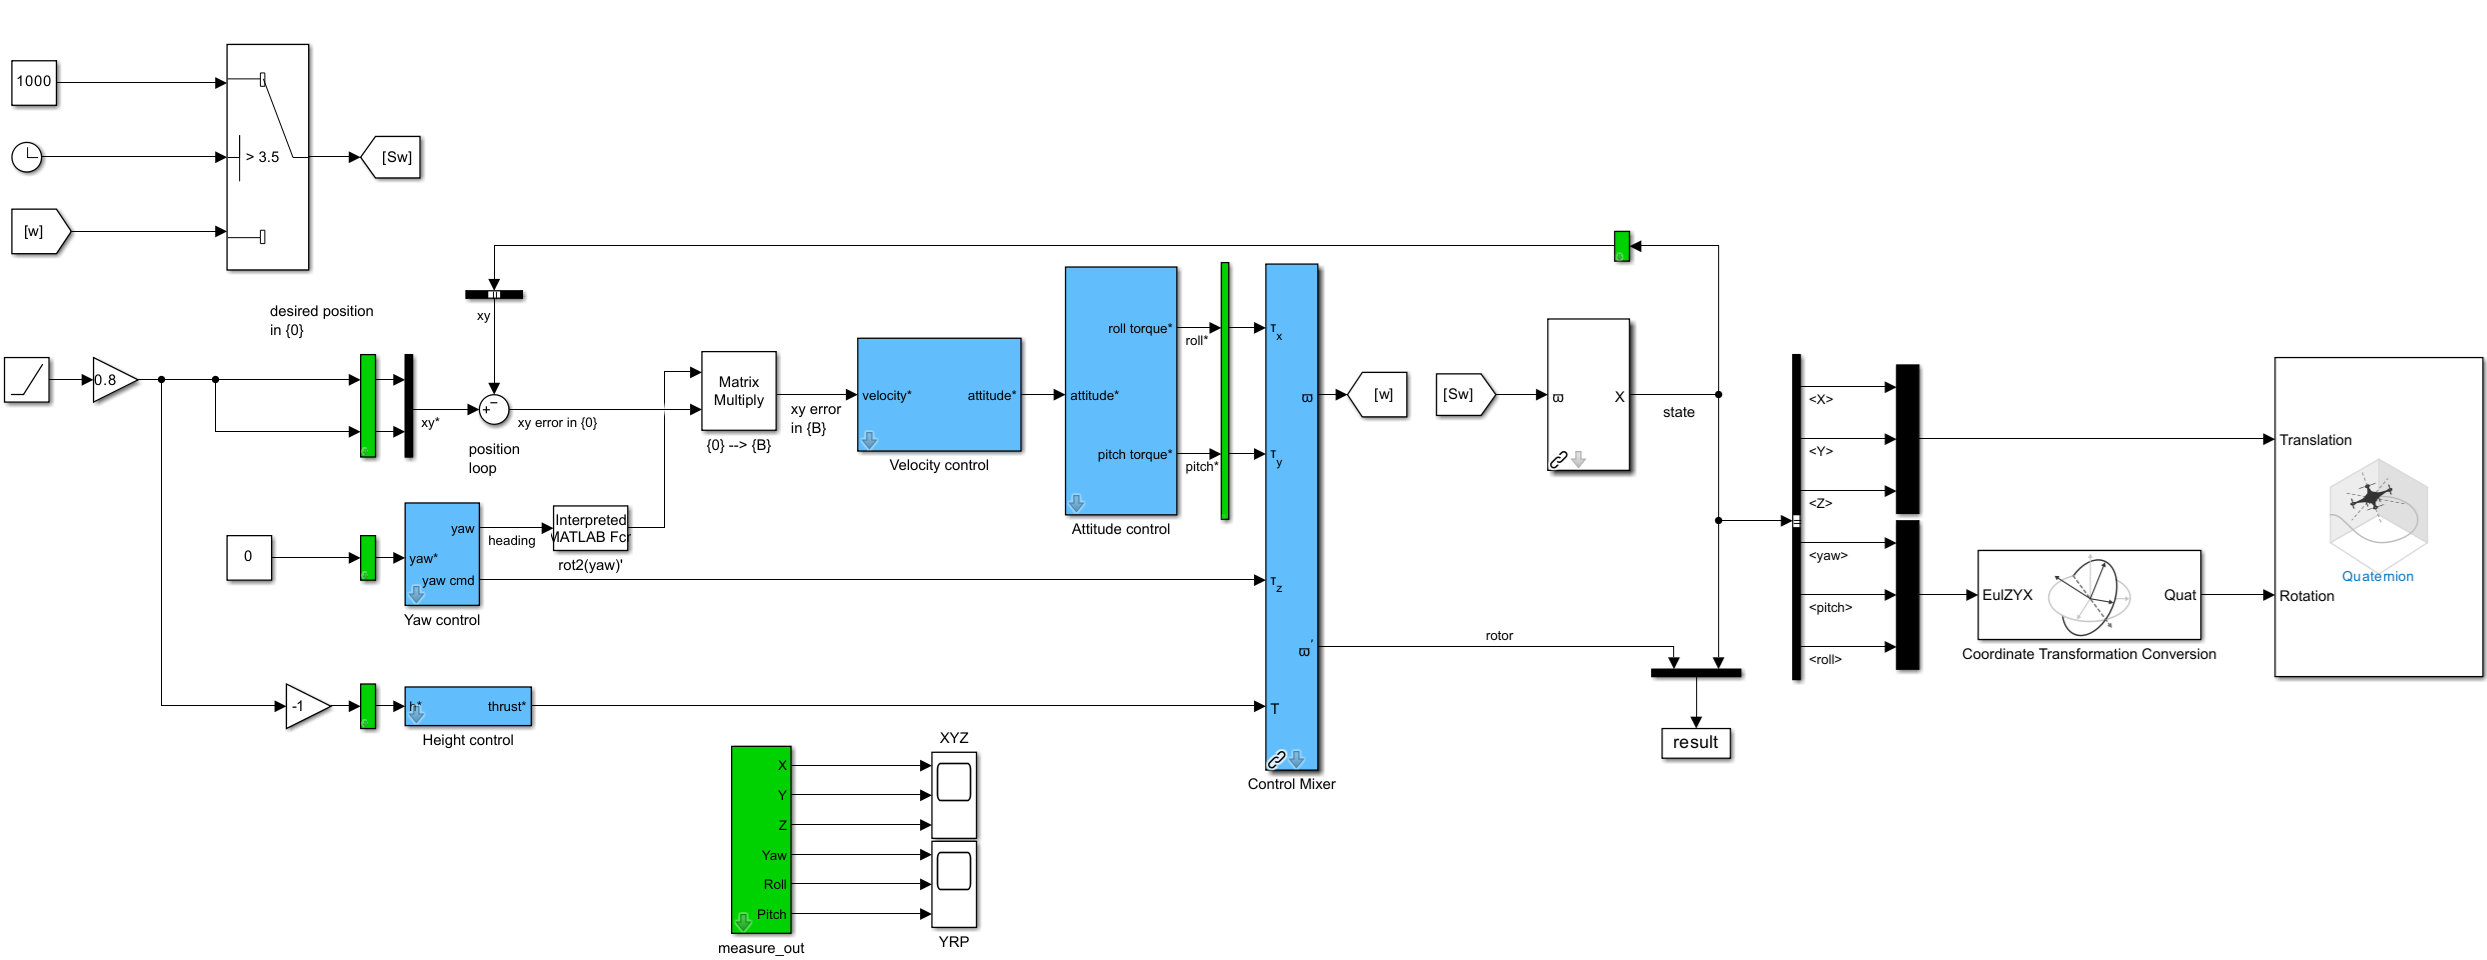
\includegraphics[width=1\linewidth]{paraboliczna/sc_parab.png}
    \caption{Schemat realizacji trajektorii balistycznej}
    \label{fig:enter-label}
\end{figure}

Ciąg generowany przez śmigła będzie ograniczoany, w różnych odstępach czasu. Badanie odległości punktu
lądowania od czasów wyłączenia, umożliwi wyprowadzenie zależności czasu ograniczenia ciągu od odległości;
ostatecznie taki zabieg umożliwi stworzenie realacji, która pozwoli zadawać punkt lądowania, Rysunek ...
Znając realcję czasu wyłączenia od odległości na jakiej ląduje dron (można obliczyć z eq...).
\begin{equation}
    s = \sqrt{x^{2}+y^{2}}
\end{equation}
Można z pomocą Rysunku ... aproksymować odległość punktu lądowania. W takim kontekście zadanie punktu lądowania powinno odpowiadać
wektorowi przemieszczenia w płaszczyźnie XY i relacji czasu ograniczenia ciągu. Pierwszą rzeczą będzie zadanie określenia kąta wektora przemieszczenia
w płaszczyźnie XY, eq\dots


\begin{equation}
    k_{x} = \sin \arctan \frac{x^{*}}{y^{*}}
\end{equation}

\begin{equation}
    k_{y} = \cos \arctan \frac{x^{*}}{y^{*}}
\end{equation}
Natomiast moduł wektora przemieszczenia określa równanie aproksymacji drogi eq ...

\begin{equation}
    t = \sqrt{x^{2}+y^{2}} - 0.13
\end{equation}

\begin{figure}[ht]
    \centering
    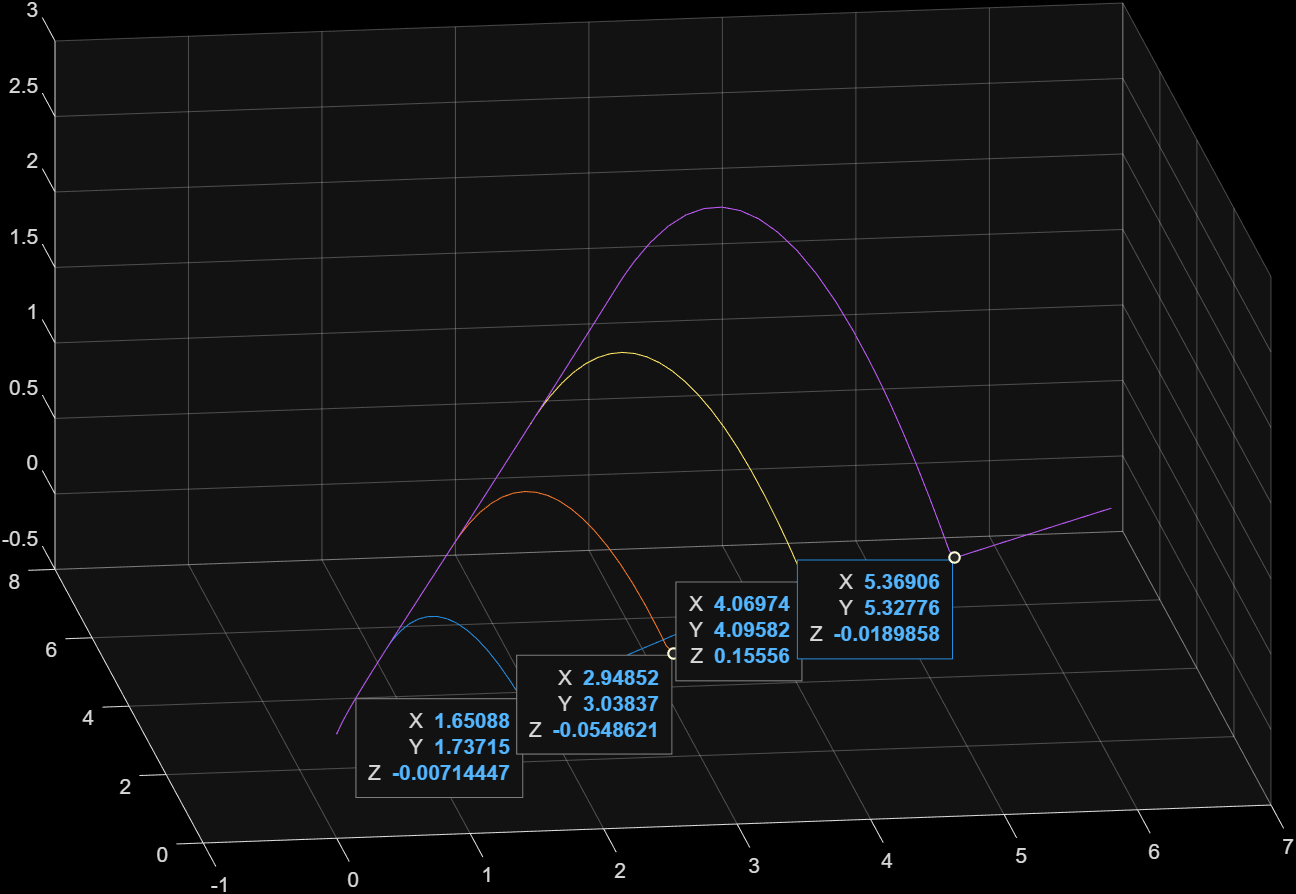
\includegraphics[width=0.7\linewidth]{paraboliczna/parabole.png}
    \caption{Otrzymane trajektorie balistyczne}
    \label{fig:enter-label}
\end{figure}

\begin{figure}[ht]
    \centering
    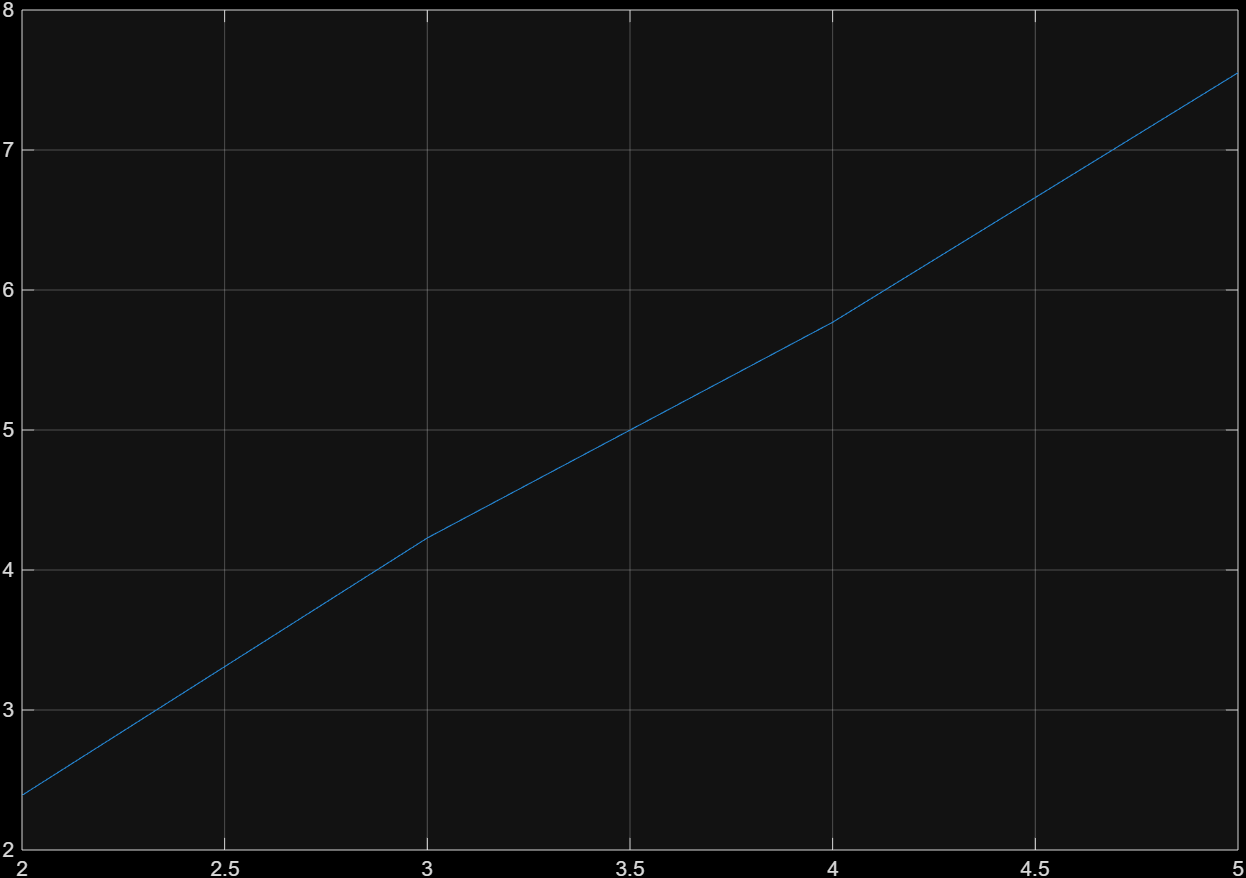
\includegraphics[width=0.7\linewidth]{paraboliczna/st.png}
    \caption{Odległość od punktu startowego}
    \label{fig:enter-label}
\end{figure}

\subsection*{Wnioski}
Wykonane badania pozwalają określić, zależności na wykonanie balistycznego lotu śmigłowca wielowirnikowego.
Zastosowanie liniowo narastających wartości zadanych umożliwia zadanie stałego przyspieszenia obiektu, natomiast
ograniczenie ciągu wymusza ruch po trajektorii balistycznej. Wykonane badanie wraz z aproksymacją umożliwia 
wyprowadzenie równań na lot balistyczny w przybliżeniu do punktu zadanego.

\section*{Zadanie nr 3}
\subsection*{Treść}
Opracuj funkcję realizującą automatyczne lądowanie śmigłowca w oparciu o dostępne 
sygnały pomiarowe (lądowanie może być aktywowane w dowolnym momencie, ze wskazaniem miejsca laowania,
po aktywowaniu funkcji automatycznego lądowania śmigłowiec przerywa wcześniej realizowany scenariusz,
podąża do punktu lądowania, przechodzi do zawisu, po czym łagodnie ląduje)

\section*{Zadanie nr 4}
\subsection*{Treść}
Zaimplementuj algorytmy planowania i śledzenia ściezek robota latającego
(Bug2, DX, D*, PRM oraz algorytmu wykorzystującego dowolnie zdefiniowane pole potencjałowe).
Mapa otoczenia jest dostarczona przez prowadzącego.



\end{document}